\model{The Die Class}

The following class represents an individual ``die'' in a game of dice.
The diagram on the right is a graphical summary of the \emph{attributes} (variables) and \emph{methods} of the class.

\vspace{1em}
\begin{quote}
\hfill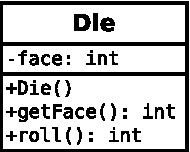
\includegraphics{Die.pdf}
\vspace*{-84pt}

\begin{javalst}
/**
 * Simulates a die object.
 */
public class Die {

    private int face;

    /**
     * Constructs a die with face value 1.
     */
    public Die() {
        this.face = 1;
    }

    /**
     * @return current face value of the die
     */
    public int getFace() {
        return this.face;
    }

    /**
     * Simulates rolling the die.
     * 
     * @return new face value of the die
     */
    public int roll() {
        this.face = (int) (Math.random() * 6) + 1;
        return this.face;
    }

}
\end{javalst}

\vspace*{-72pt}
% https://commons.wikimedia.org/wiki/File:2-Dice-Icon.svg
\hfill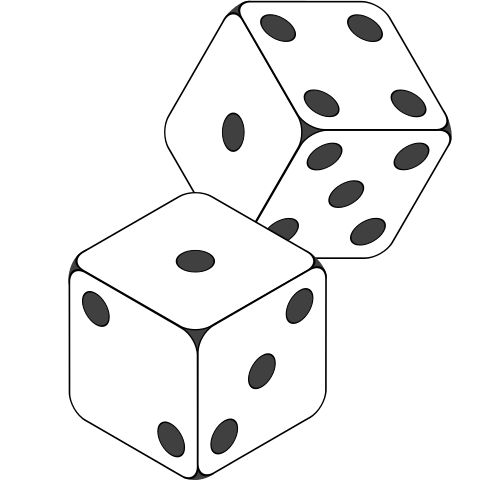
\includegraphics[width=2in]{dice.png}
\end{quote}


\newpage
\quest{10 min}


\Q Consider the \java{Die} class:

\begin{enumerate}
\item What are the attributes?
\ans[10em]{face}

\item What are the methods?
\ans[10em]{Die, getFace, roll}
\end{enumerate}


\Q In the class diagram (on the upper right):

\begin{enumerate}
\item What do the \java{+} and \java{-} symbols represent?
\ans[18em]{\jans{+} means \jans{public} ~ \jans{-} means \jans{private}}

\item What does the \java{:} represent?
\ans[18em]{the data type of the attribute/method}
\end{enumerate}


\Q Open the provided \textit{Die.java} and run the program several times.
Then answer the following questions about the \java{main} method:
\begin{enumerate}
\item What is the data type of \java{d1} and \java{d2}?
\ans[8em]{Die}

\item What are the initial values of the dice?
\ans[8em]{d1 = 1, d2 = 1}

\item What method changed the dice values?
\ans[8em]{roll}
\end{enumerate}


\Q \label{dievar}
Write a statement that declares and initializes a \java{Die} variable named \java{lucky}.
%(Do not initialize the variable.)

\begin{answer}[3em]
\tt Die lucky = new Die();
\end{answer}


%\Q Write a statement that creates a new \java{Die} and assigns it to \java{lucky}.
%(Do not declare the variable.)
%
%\begin{answer}[2em]
%\tt lucky = new Die();
%\end{answer}


\Q When you create an object, Java invokes a \emph{constructor}.
This method has no return type and has the same name as the class itself.
What does the \java{Die()} constructor do?

\begin{answer}
It initializes the \java{face} attribute to 1.
(Without this constructor, the default value would be 0, which is invalid for dice.)
\end{answer}


\Q Notice how the \java{roll} method refers to \java{this.face}, yet that variable is not declared in the method. What does the \java{roll} method change, in terms of the \java{Die} object?

\begin{answer}[3em]
It updates the value of the \java{face} attribute.
\end{answer}


%\Q What is the purpose of the \java{getFace} method?
%Show how you would use it in a \java{main} method of another class.
%
%\begin{answer}[3em]
%In a {\tt main} method, you would do something like: {\tt System.out.println(lucky.getFace());}
%\end{answer}
